% Gemini theme
% https://github.com/anishathalye/gemini
% Poster for: Perceptual and Acoustic Correlates of Racial Identity in Text-to-Speech Voices

\documentclass[final,20pt]{beamer}

% ====================
% Packages
% ====================

\usepackage[size=custom,width=122,height=92,scale=0.88]{beamerposter}
\usetheme{gemini}
\usecolortheme{amp}
\usepackage{graphicx}
\usepackage{booktabs}
\usepackage{tabularx}
\usepackage{multicol}
\usepackage{multirow}
\usepackage{array}
\usepackage{caption}
\usepackage{adjustbox}
\usepackage{xspace}
\usepackage{anyfontsize}

\usepackage[round]{natbib}
\bibpunct[:\ ]{(}{)}{,}{a}{}{,}
\usepackage{natbibspacing}		% single-space bibliography
\bibliographystyle{unified}
\newcommand{\etal}{et al.\xspace}

\usepackage{paralist}

\renewenvironment{thebibliography}[1]{%
\textbf{References cited.}%
\let\par\relax\let\newblock\relax%
\let\oldbibitem\bibitem%
\newif\iffirstbib\firstbibtrue%
\def\bibitem{\iffirstbib\firstbibfalse\else\unskip\ \textbullet~~\fi\oldbibitem}%
\inparaitem[{[}1{]}]}{\endinparaitem}

\definecolor{lightgray}{RGB}{245, 246, 250}
\definecolor{darkblue}{HTML}{2D728F}
\definecolor{blue}{HTML}{429eb8}
\definecolor{yellow}{HTML}{F4F0E6}
\definecolor{orange}{HTML}{F49E4C}
\definecolor{red}{HTML}{84271E}

% IPA symbols are typed directly in Unicode (æ ɛ ɪ ɑ aɪ eɪ)
\newcommand{\ipa}[1]{\textit{/#1/}}

% ====================
% Lengths
% ====================

\newlength{\sepwidth}
\newlength{\colwidth}
\setlength{\sepwidth}{0.025\paperwidth}
\setlength{\colwidth}{0.3\paperwidth}
\newcommand{\separatorcolumn}{\begin{column}{\sepwidth}\end{column}}

% ====================
% Title
% ====================

\title{Perceptual and Acoustic Correlates of Racial Identity \\ in Text-to-Speech Voices}
\author{Noah Khaloo\textsuperscript{1}, Nicole Holliday\textsuperscript{2}, Sarah Creel\textsuperscript{1}}
\email{nkhaloo@ucsd.edu, nicole.holliday@berkeley.edu, screel@ucsd.edu}
\institute[shortinst]{\textsuperscript{1}UC San Diego \quad \textsuperscript{2}UC Berkeley}

% ====================
% Footer
% ====================

\footercontent{%
  \hfill Interspeech 2026 \hfill
}

\begin{document}
\renewcommand{\arraystretch}{1.15}
\begin{frame}[t]
\begin{columns}[t]
\separatorcolumn

% ==================================================================
% COLUMN 1
% ==================================================================
\begin{column}{\colwidth}

\begin{block}{~BACKGROUND}

    \begin{itemize}
        \item Listeners recover \textbf{race} from voice alone: American English listeners reliably distinguish White and Black speakers from phonetic cues of Mainstream American English (MAE) vs.\ African American English (AAE) \citep{purnell_perceptual_1999,thomas_delimiting_2004} --- and judge voices heard as `sounding Black' \textbf{more negatively}.
        \item Voice-AI is increasingly human-like and deployed in high-stakes settings, but findings on race in TTS are \textbf{mixed}: listeners converge on race labels \citep{holliday_siri_2023}, yet show a bias towards rating synthetic voices as `White' \citep{pinhanez_harnessing_2024}.
    \end{itemize}

    \vspace{.5em}
    \textbf{Research questions}
    \begin{itemize}
        \item[\textbf{Q1}] Can listeners perceive race in \textbf{fully synthetic} voices they know are synthetic?
        \item[\textbf{Q2}] Does perceived race interact with \textbf{personality} judgments, and with perceived \textbf{human-likeness}?
        \item[\textbf{Q3}] Which \textbf{acoustic features} distinguish Black- from White-rated voices?
    \end{itemize}

\end{block}

\begin{block}{~METHODS}

    \textbf{Perception experiment}
    \begin{itemize}
        \item \textbf{144} American English listeners (Prolific), ethnically representative sample; \textbf{32 TTS voices} (EasyPeasy AI): 8 per platform-assigned label --- \{Black, White\} $\times$ \{Male, Female\}. Audio only, amplitude-normalized to 72\,dB.
        \item \textbf{Personality block:} 16 voices read the Rainbow Passage; 7-point ratings for \textit{friendly, professional, competent, trustworthy, pleasant, funny} $+$ \textbf{human-likeness} \citep{holliday_siri_2023}.
        \item \textbf{Race block:} the other 16 voices; 4 sentences targeting AAE-relevant vowels (\ipa{æ, ɛ, ɪ, i, ɑ, eɪ, aɪ}), avoiding AAE morphosyntactic cues; forced-choice race (Asian, Black, Hispanic/Latino, White) $+$ age, region, gender; 64 trials.
    \end{itemize}

    \vspace{.5em}
    \textbf{Acoustic features} \hfill {\footnotesize \citep[Psychoacoustic Model of the Voice;][]{kreiman_toward_2014}}
    \begin{itemize}
        \item Per vowel token, at 1-ms frames (VoiceSauce; \citealt{Shue2009}): F0, \textbf{F1--F4}, formant dispersion; \textbf{Residual H1*}, H2*--H4*, H4*--H2kHz*, H2kHz*--H5kHz*; \textbf{CPP}, SHR, Energy.
        \item MAD outlier exclusion; min--max normalization within gender; \textbf{mean $+$ CoV} at vowel onset/midpoint/offset; centered by phonation modality.
    \end{itemize}

    \vspace{.5em}
    \textbf{Classifier}
    \begin{itemize}
        \item \textbf{Gradient Boosted Decision Trees} (XGBoost; \citealt{chen2024}) classify Black- vs.\ White-rated voices from 61 features; speaker-level 5-fold cross-validation $\times$ 50 repeats, grid-searched hyper-parameters.
    \end{itemize}

\end{block}

\begin{alertblock}{}
    \scriptsize{%
    \bibliography{poster.bib}%
    }
\end{alertblock}

\end{column}

\separatorcolumn

% ==================================================================
% COLUMN 2
% ==================================================================
\begin{column}{\colwidth}

\begin{block}{~PERCEPTUAL RESULTS: RACE}

    \begin{itemize}
        \item Agreement with platform-assigned \textbf{gender} was near ceiling (Male: 98.6\%; Female: 93.6\%).
        \item Perceptually grounded \textbf{race labels} derived by k-means clustering on \%~Reported Black (RB): voices consistently rated \textbf{White} ($\sim$0--20\% RB), \textbf{Ambiguous} ($\sim$20--50\%), or \textbf{Black} ($\sim$50--100\%).
    \end{itemize}

    \begin{figure}
        \centering
        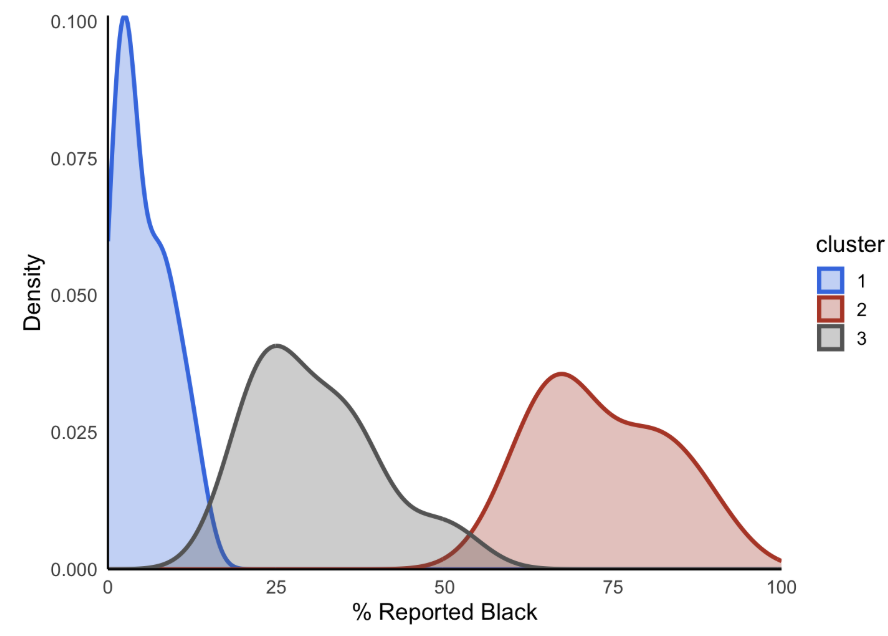
\includegraphics[width=.56\colwidth]{figures/3cluster.png}
        \caption*{\small \textit{Kernel density estimates of \% Reported Black, by cluster assignment.}}
    \end{figure}

    \begin{itemize}
        \item The Black-rated cluster is much \textbf{wider} $\rightarrow$ more rater variability, and an overall \textbf{bias towards rating voices as White}.
        \item \textbf{5/9} Ambiguous voices were platform-labeled \textit{Black Female}: Black female voices are harder to identify, as with human voices \citep{thomas_delimiting_2004}.
    \end{itemize}

\end{block}

\begin{block}{~PERCEPTUAL RESULTS: PERSONALITY}

    \begin{figure}
        \centering
        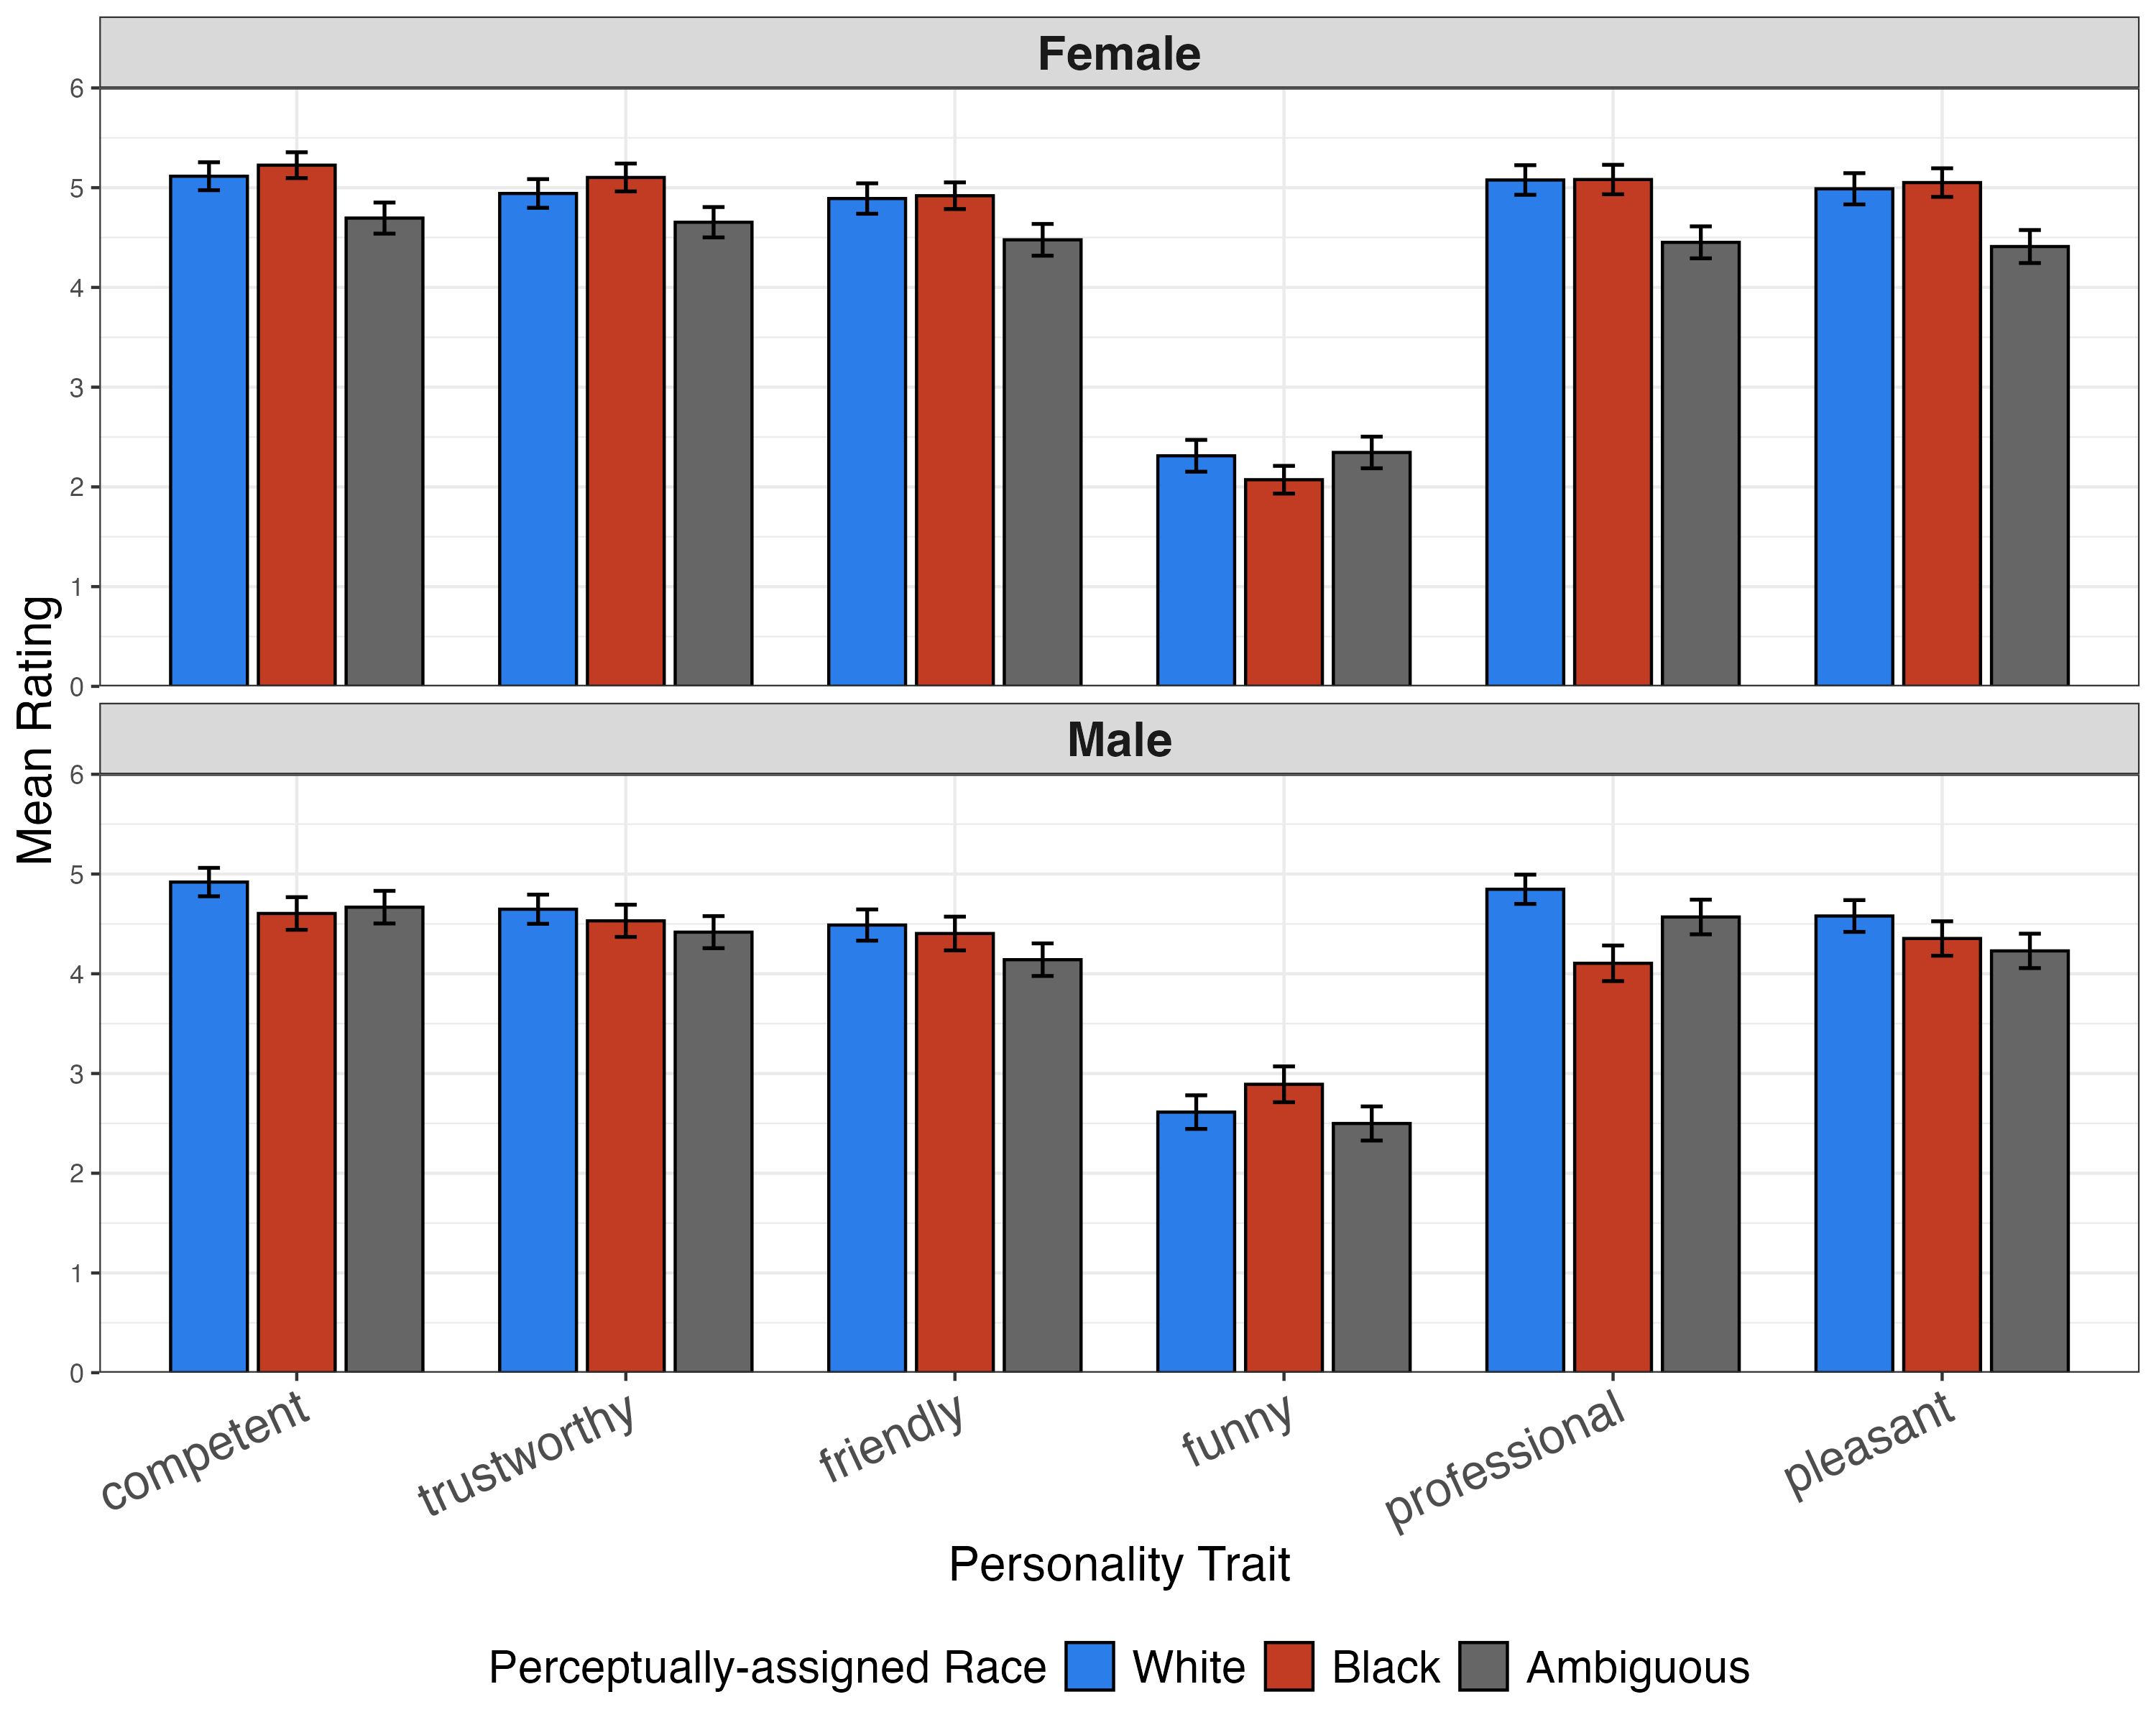
\includegraphics[width=.66\colwidth]{figures/pers_ratings.png}
        \caption*{\small \textit{Mean personality ratings by perceptually-assigned race and gender.}}
    \end{figure}

    \begin{itemize}
        \item Per-trait linear mixed-effects models: perceived race $+$ participant ethnicity $+$ human-likeness; random intercepts for participant and voice; fit separately by perceived gender.
        \item \textbf{Female voices:} no effect of perceived race on any trait. \textbf{Male voices rated Black} were rated as less \textit{pleasant} ($\beta = -0.64$), \textit{professional} ($\beta = -1.09$), \textit{trustworthy} ($\beta = -0.53$), and \textit{competent} ($\beta = -0.67$), all $p < .05$ $\rightarrow$ \textbf{racial stereotyping of synthetic voices}.
        \item \textbf{Human-likeness} positively predicted \textbf{all} traits for both genders ($p < .01$); participant ethnicity was never significant.
    \end{itemize}

\end{block}

\end{column}

\separatorcolumn

% ==================================================================
% COLUMN 3
% ==================================================================
\begin{column}{\colwidth}

\begin{block}{~ACOUSTIC RESULTS}

    \begin{itemize}
        \item Ambiguous voices excluded; classifier trained on \textbf{male-rated} voices (too few Black Female voices after filtering). Full model: \textbf{65\%} CV accuracy; reduced top-15-feature model: \textbf{66\%}.
        \item \textbf{Black-rated voices} show lower \textbf{CPP}, \textbf{H2*--H4*}, and \textbf{H2kHz*--H5kHz*}, higher \textbf{F4}, and markedly lower \textbf{Residual H1*} --- the most robust effect, linked to glottal constriction \citep{chai_h1h2_2022}.
    \end{itemize}

    \begin{figure}
        \centering
        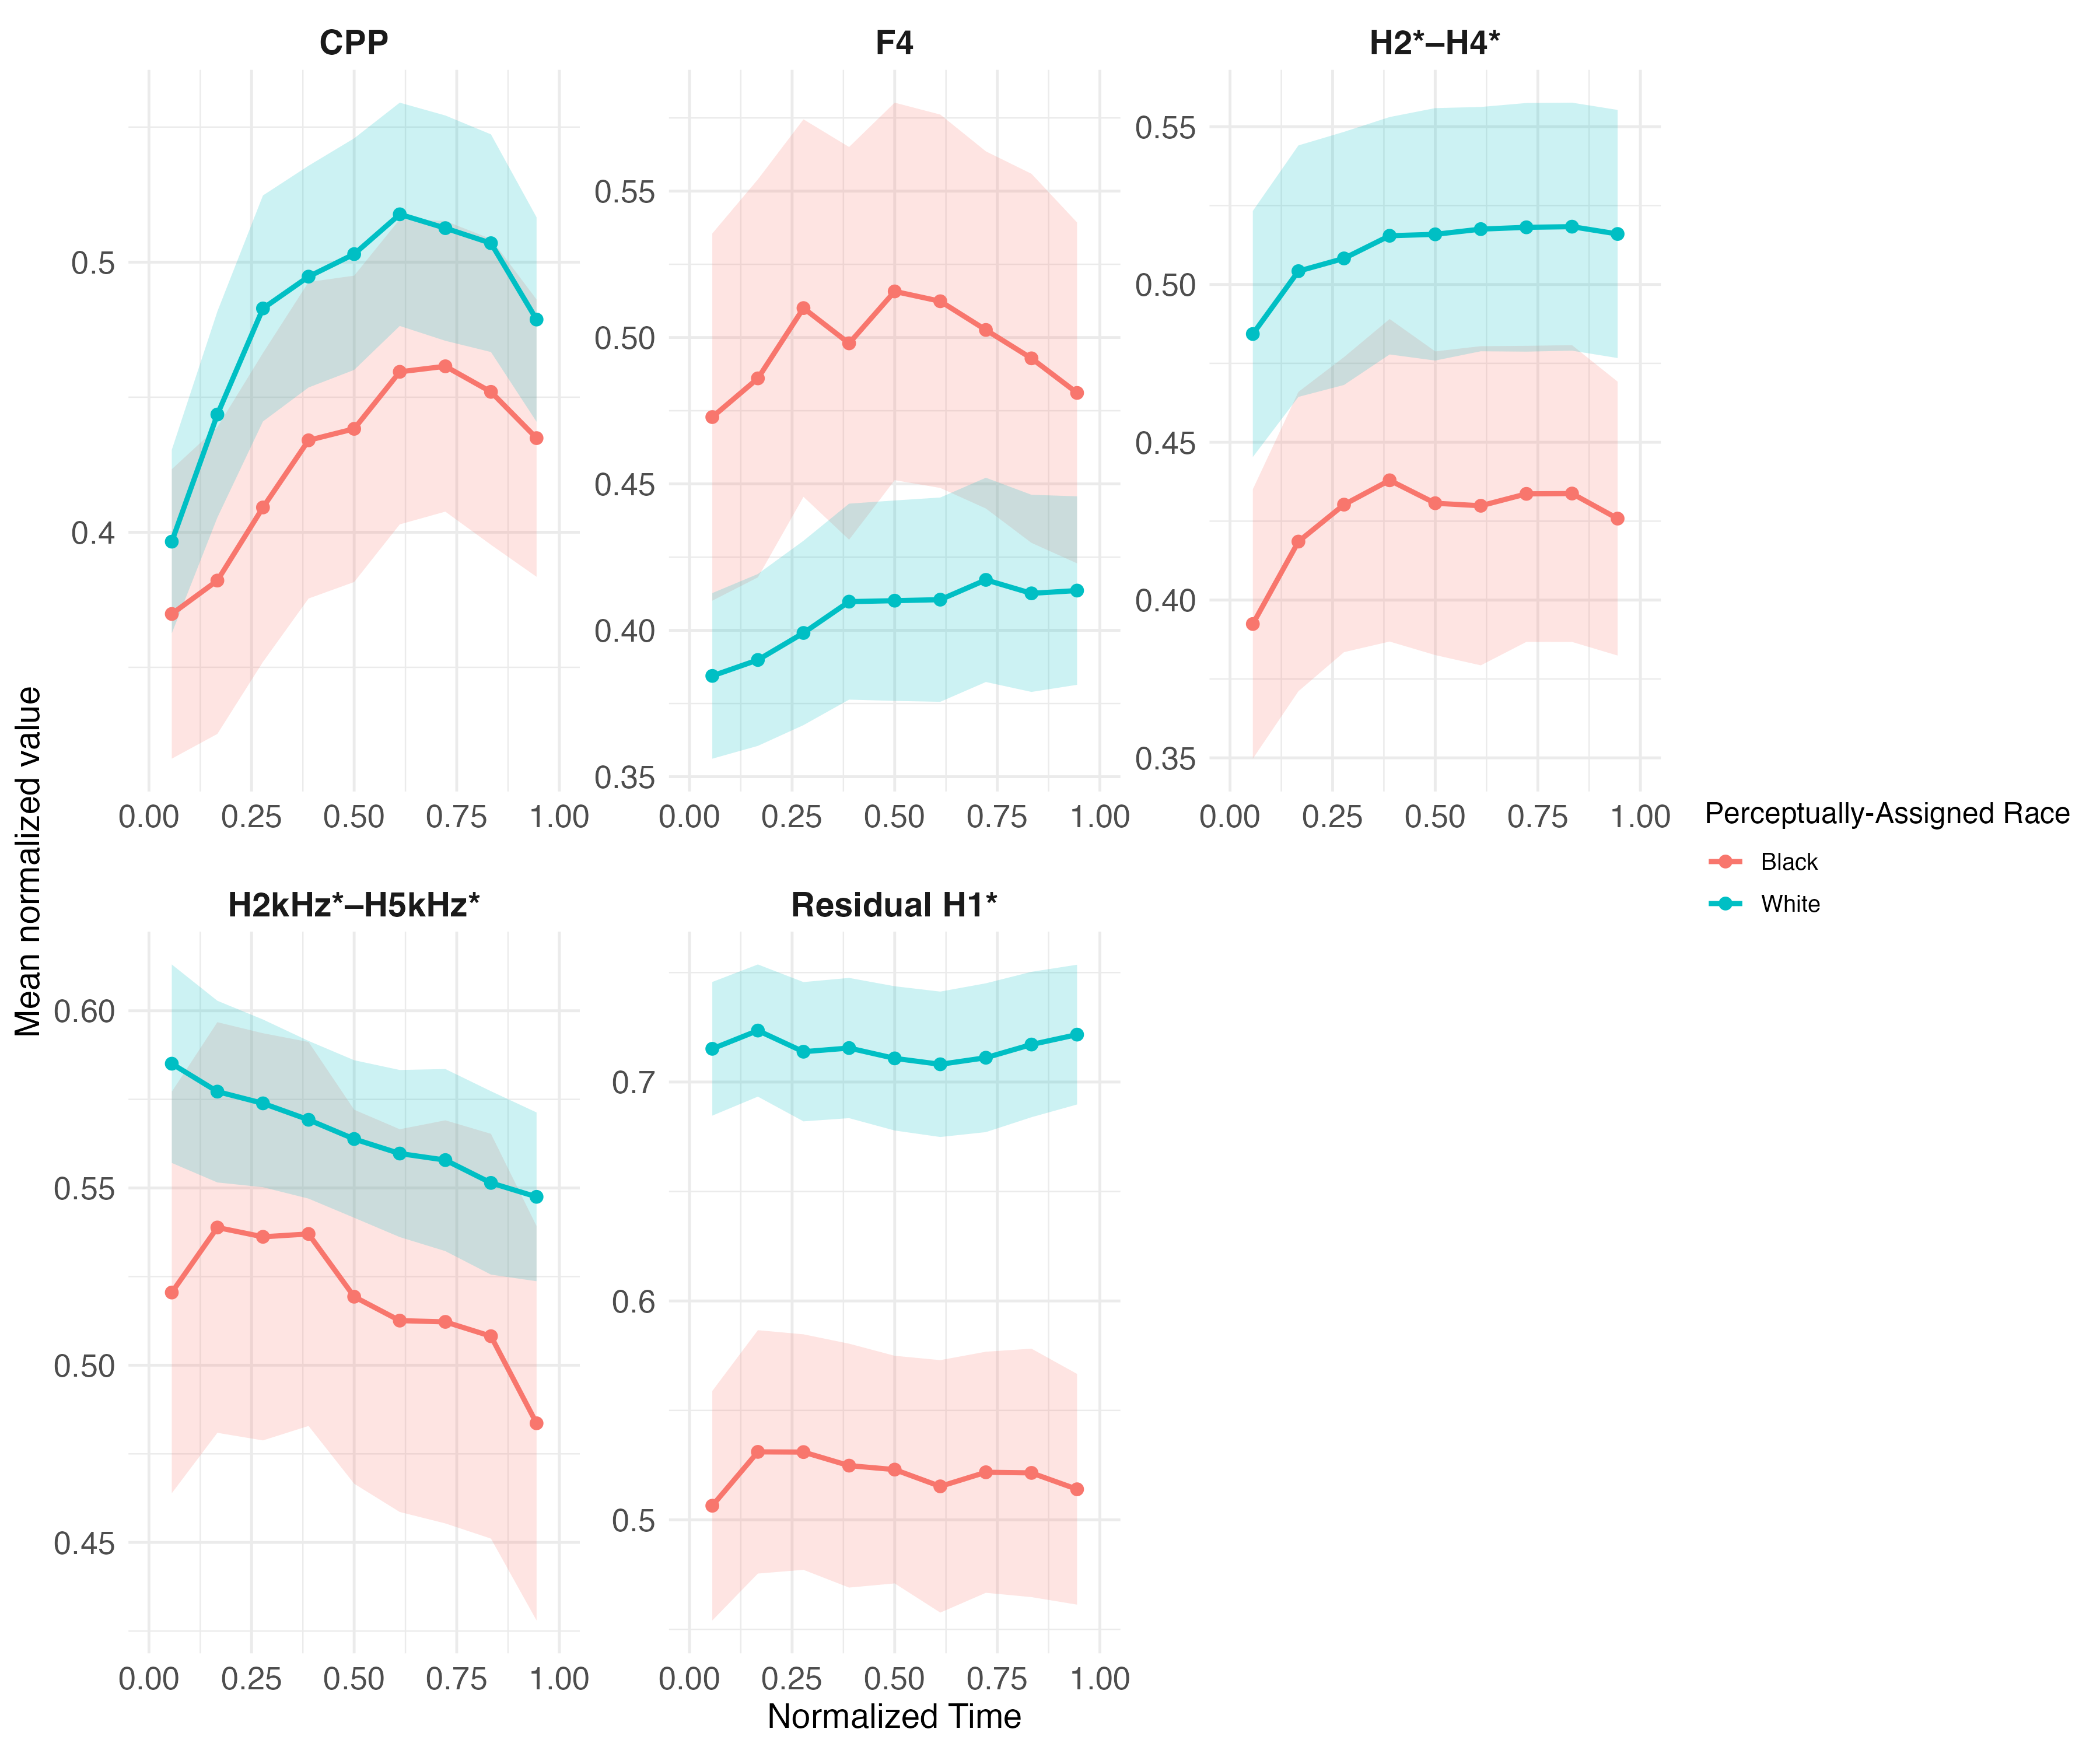
\includegraphics[width=.56\colwidth]{figures/mean_structure.png}
        \caption*{\small \textit{Mean structure across normalized time for the top classifier features (\textcolor{red}{red $=$ Black-rated}, \textcolor{darkblue}{teal $=$ White-rated}); ribbons $=$ 95\% CI.}}
    \end{figure}

    \begin{itemize}
        \item \textbf{Vowel quality:} localized $\sim$100\,Hz F1 differences for \ipa{æ, ɛ, i}, and F1/F2 differences for \ipa{aɪ} --- mirroring documented AAE--MAE vowel differences in human speech \citep{kohn_adolescent_2013}.
    \end{itemize}

    \begin{figure}
        \centering
        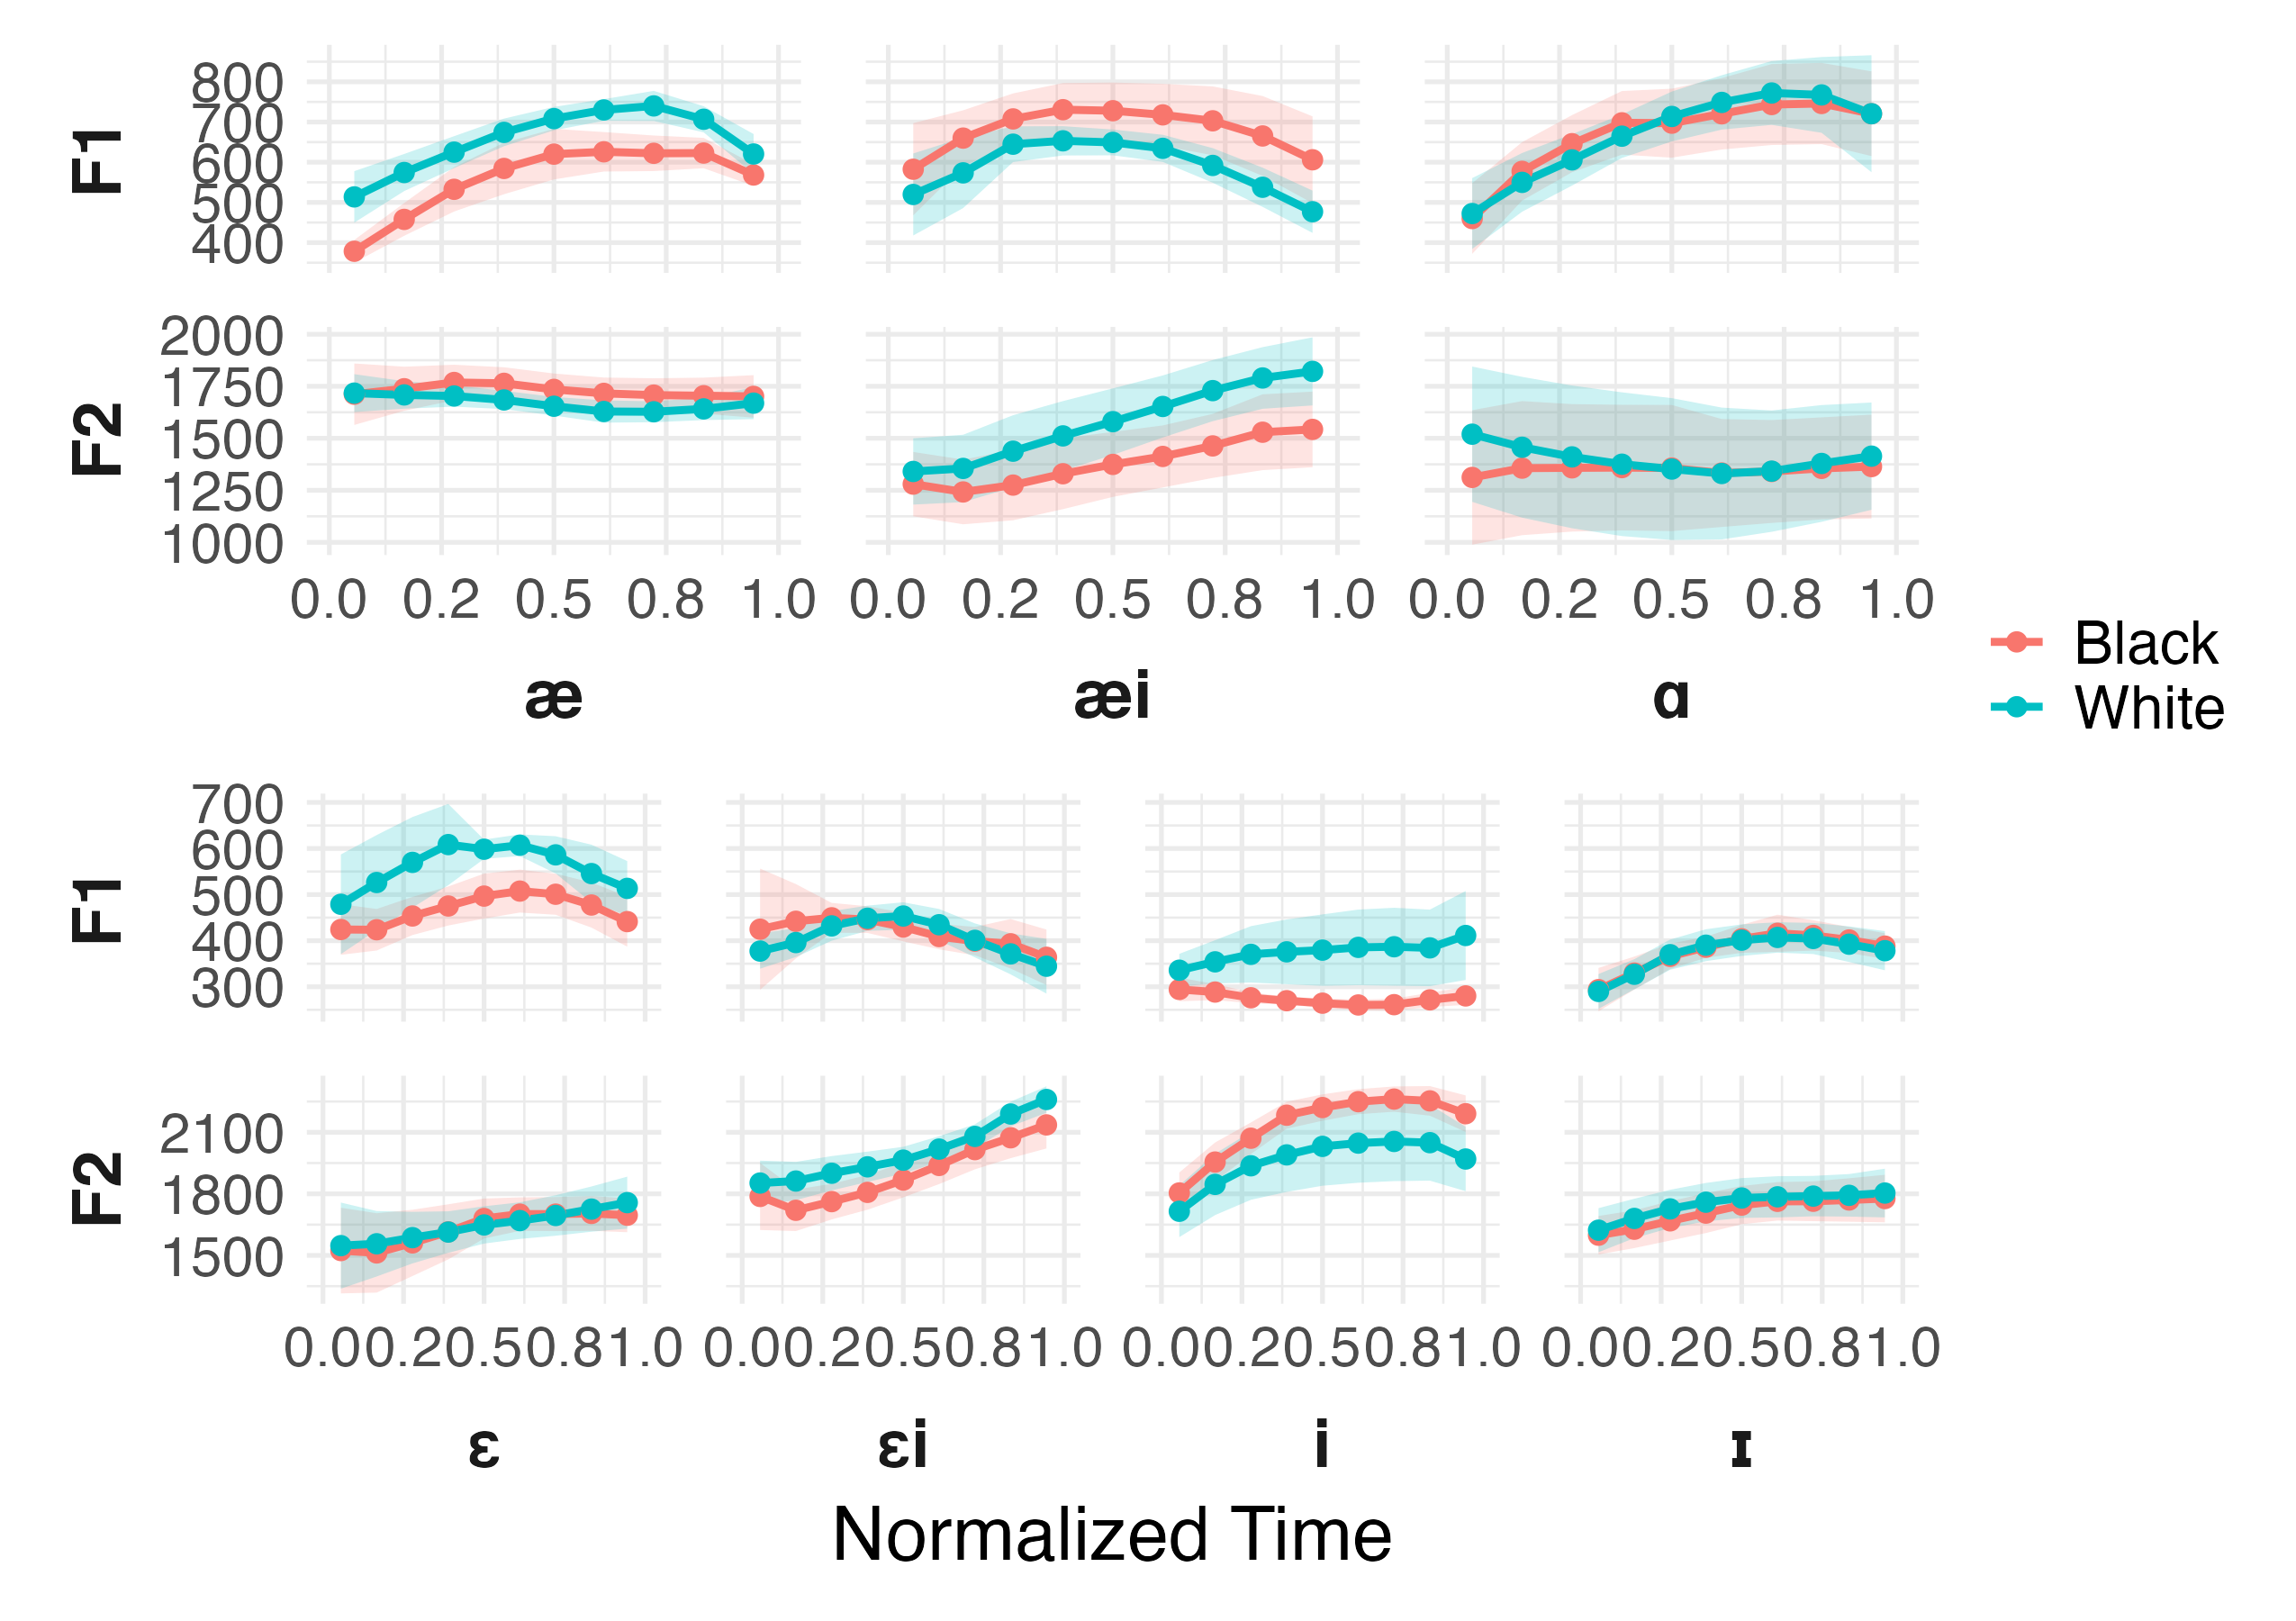
\includegraphics[width=.56\colwidth]{figures/formants.png}
        \caption*{\small \textit{Raw F1/F2 trajectories for Black- vs.\ White-rated voices; ribbons $=$ 95\% CI.}}
    \end{figure}

\end{block}

\begin{block}{~DISCUSSION}

    \begin{itemize}
        \item[\textbf{(Q1)}] Listeners \textbf{can} perceive race in fully synthetic speech, though with a bias towards `White' ratings.
        \item[\textbf{(Q2)}] Listeners \textbf{still stereotype}: male voices rated Black receive lower personality ratings, and human-likeness boosts all personality attributions (anthropomorphism) \citep{schreibelmayr_robot_2022}.
        \item[\textbf{(Q3)}] Cues tied to laryngeal configuration (\textbf{Residual H1*}, H2*--H4*), speaker individuality (CPP, F4; \citealt{lee_acoustic_2019}), and \textbf{AAE-like vowel quality} distinguish Black- from White-rated voices.
        \item[] \textbf{Implications:} these acoustics can guide the design of racially-marked voices, but stereotyping warrants \textbf{caution} when deploying synthetic speech in socially sensitive contexts.
    \end{itemize}

\end{block}

\end{column}

\separatorcolumn
\end{columns}

\end{frame}

\end{document}
